\subsection{Operation Model for oeAlert}

\label{OM-oeAlert}


The \msrcode{oeAlert} operation has the following properties:

	\begin{operationmodel}
	\addheading{Operation}
	\adddoublerow{oeAlert}{Any human having a phone able to connect to the communication companies using the \msricrash system can send his company an sms message with structured information in order to declare an alert.}

	\addrowheading{Parameters}
	\addnumbereddoublerow{}{AetHumanKind: etHumanKind}{the kind of human informing of an alert.} 
	\addnumbereddoublerow{}{AdtDate: dtDate}{the date of the alert } 
	\addnumbereddoublerow{}{AdtTime: dtTime}{the time of the alert} 
	\addnumbereddoublerow{}{AdtPhoneNumber: dtPhoneNumber}{the phone number of the human sending the alert SMS message } 
	\addnumbereddoublerow{}{AdtGPSLocation: dtGPSLocation}{ the GPS position of the phone at the date and time the message was sent.} 
	\addnumbereddoublerow{}{AdtComment: dtComment}{a free text message sent by the human providing information on the alert that he wants to declare} 
	\addnumbereddoublerow{}{AetKind: etHumanKind}{ } 
	\addnumbereddoublerow{}{AdtMyDate: dtDate}{ } 
	\addnumbereddoublerow{}{AdtTime: dtTime}{ } 
	\addnumbereddoublerow{}{AdtPhoneNumber: dtPhoneNumber}{ } 
	\addnumbereddoublerow{}{AdtGPSLocation: dtGPSLocation}{ } 
	\addnumbereddoublerow{}{AdtComment: dtComment}{ } 

	\addrowheading{Return type}
	\addsinglerow{ptBoolean}

	\addrowheading{Pre-Condition (protocol)}
	\addnumberedsinglerow{PreP}{ the system is supposed to be created and initialized.}
		
	\addrowheading{Pre-Condition (functional)}
	\addnumberedsinglerow{PreF}{ the date and time the alert is declared is supposed to be in the past with respect to the current time known by the system.}

	\addrowheading{Post-Condition (functional)}
	\addnumberedsinglerow{PostF}{ the ctState attribute for the next value for alert IDs is incremented by one at post.}
	\addnumberedsinglerow{PostF}{ a new alert instance exists in the post state with status pending, instant information (resp. GPS location and comment) based on date and time provided (resp. position and comment); and with alert ID being a string conversion of the dtInteger value available in the pre state in the ctState instance.}
	\addnumberedsinglerow{PostF}{if there exist no already registered alert near to the alert currently declared
	then a new crisis is added in the post state and initialized with: its ID being the one provided by the ctState instance (which is incremented by one in the post state), its type considered as small, its status being pending, its declared time being the same than the alert and a default comment indicating that a report will come later on.
	else the crisis to which the new alert must be related to is the one related to any alert nearby in the pre-state.}
	\addnumberedsinglerow{PostF}{the post state relates the new alert to the previously characterized crisis.}
	\addnumberedsinglerow{PostF}{if there is no ctHuman instance having same phone number and same kind in the pre-state 
	then a new one is added in the post-state with given phone number and kind and is associated to the communication company actor used to declare the alert.
	else the pre-state one is chosen
	}
	\addnumberedsinglerow{PostF}{and this specified ctHuman is related to the new alert thus indicating he has signed the alert. }
	\addnumberedsinglerow{PostF}{A new ctAlertBackup is created, with the same attributes that the ctAlert has}

	\addrowheading{Post-Condition (protocol)}
	\addnumberedsinglerow{PostP}{ none}
	\end{operationmodel}



	% ------------------------------------------
	% MCL Listing
	% ------------------------------------------
	\vspace{1cm}
	The listing~\ref{OM-actComCompany-oeAlert-MCL-LST} provides the \msrmessir (MCL-oriented) specification of the operation.
	
	\scriptsize
	\vspace{0.5cm}
	\begin{lstlisting}[style=MessirStyle,firstnumber=auto,captionpos=b,caption={\msrmessir (MCL-oriented) specification of the operation \emph{oeAlert}.},label=OM-actComCompany-oeAlert-MCL-LST]

	/* Pre Protocol:*/ 
	preP{let TheSystem: ctState in
	  self.rnActor.rnSystem = TheSystem
	  
	/* PreP01 */
	  and TheSystem.vpStarted = true}
	
	/* Pre Functional:*/
	preF{let TheSystem: ctState in
	  self.rnActor.rnSystem = TheSystem
	
	/* PreF01 */
	  and (TheSystem.clock.date.gt(AdtDate)
	       or (TheSystem.clock.date.eq(AdtDate)
	           and TheSystem.clock.time.gt(AdtTime)
	          )
	      )}
	
	/* Post Functional:*/ 
	postF{let TheSystem: ctState in
	  
	 let  ActHuman:ctHuman in
	 let  TheactComCompany:actComCompany in
	 let  ActAlert:ctAlert in
	 let  AAlertInstant:dtDateAndTime in
	 let  AetAlertStatus:etAlertStatus in
	 let  ActAlertNearBy:ctAlert in
	 let  ActCrisis:ctCrisis in
	 let  AdtCrisisID:dtCrisisID in
	 let  AetCrisisType:etCrisisType in
	 let  AetCrisisStatus:etCrisisStatus in
	 let  ACrisisInstant:dtDateAndTime in
	 let  ACrisisdtComment:dtComment in
	 let  AptStringMessage:ptString in
	 let  AdtSMS:dtSMS in
	 let  AdtAlertID:dtAlertID in
	 let  ActAlertBackup:ctAlertBackup in
	 
	  self.rnActor.rnSystem = TheSystem
	  and self.rnActor = TheactComCompany
	/* PostF01 */
	 TheSystem.nextValueForAlertID=PrenextValueForAlertID
	 and PrenextValueForAlertID.add(1) = PostnextValueForAlertID
	 and TheSystem@post.nextValueForAlertID = PostnextValueForAlertID
	
	
	  /* PostF02 */
	and AAlertInstant.date=AdtDate
	and AAlertInstant.time=AdtTime
	
	and AetAlertStatus=pending
	        
	and TheSystem.nextValueForAlertID.todtString().eq(AdtAlertID)
	
	and ActAlert.init(AdtAlertID,
	                  AetAlertStatus,
	                  AdtGPSLocation,
	                  AAlertInstant,
	                  AdtComment)
	
	and ActAlert@post.hash = ActAlert.hash.calculate(AdtAlertID, AdtGPSLocation, AdtComment, AAlertInstant)
	      
	  /* PostF03 */
	and TheSystem.rnctAlert.select(location.isNearTo(AdtGPSLocation)) = ColctAlertsNearBy
	and if  (ColctAlertsNearBy->size()=0)
	    then (TheSystem.nextValueForCrisisID = PrenextValueForCrisisID
	          and PrenextValueForCrisisID.add(1) = PostnextValueForCrisisID
	          and TheSystem@post.nextValueForCrisisID = PostnextValueForCrisisID
	          and TheSystem.nextValueForCrisisID.todtString().eq(AdtCrisisID)
	          and AdtCrisisType = small
	          and AetCrisisStatus = pending
	          and ACrisisInstant= AAlertInstant
	          and ACrisisdtComment = 'no reporting yet defined'
	          and ActCrisis.init( AdtCrisisID,
	                              AdtCrisisType,
	                              AetCrisisStatus,
	                              AdtGPSLocation,
	                              ACrisisInstant,
	                              ACrisisdtComment)
	         )
	  else (ColctAlertsNearBy.rnTheCrisis->msrAny(true) = ActCrisis)
	  endif
	
	  /* PostF04 */
	and ActAlert@post.rnTheCrisis = ActCrisis
	      
	/* PostF05 */
	and  TheSystem.rnctHuman->select(id.eq(AdtPhoneNumber)) = HumanCol1
	
	and HumanCol1->select(kind.etEq(AetHumanKind)) = HumanCol2
	and if (HumanCol2->msrIsEmpty)
	    then (ActHuman.init(AdtPhoneNumber,AetHumanKind)
	          and ActHuman@post.rnactComCompany = TheactComCompany
	         )
	    else (HumanCol2->any(true) = ActHuman)
	    endif
	    
	 and ActHuman.rnSignaled->msrIncluding(ActAlert) = ColAlerts
	 
	 and ActHuman@post.rnSignaled = ColAlerts
	
	/* PostF06 */
	AdtSMS.value = 'Your alert has been registered. We will handle it and keep you informed'
	and TheactComCompany.rnInterfaceIN^ieSmsSend(AdtPhoneNumber,AdtSMS)
	
	/* PostF07 */
	and ActAlertBackup.init(AdtAlertID,
	                  AetAlertStatus,
	                  AdtGPSLocation,
	                  AAlertInstant,
	                  AdtComment)}
	
	/* Post Protocol:*/ 
	postP{ true}
	
	\end{lstlisting}
	\normalsize 
	
	
	
	





Figure \ref{fig:lu.uni.lassy.excalibur.examples.icrash-OM-scopeView-operation-scope-outactComCompany-oeAlertv2}
shows concept model elements in the scope of the oeAlert operation

\begin{figure}[htbp]
\begin{center}

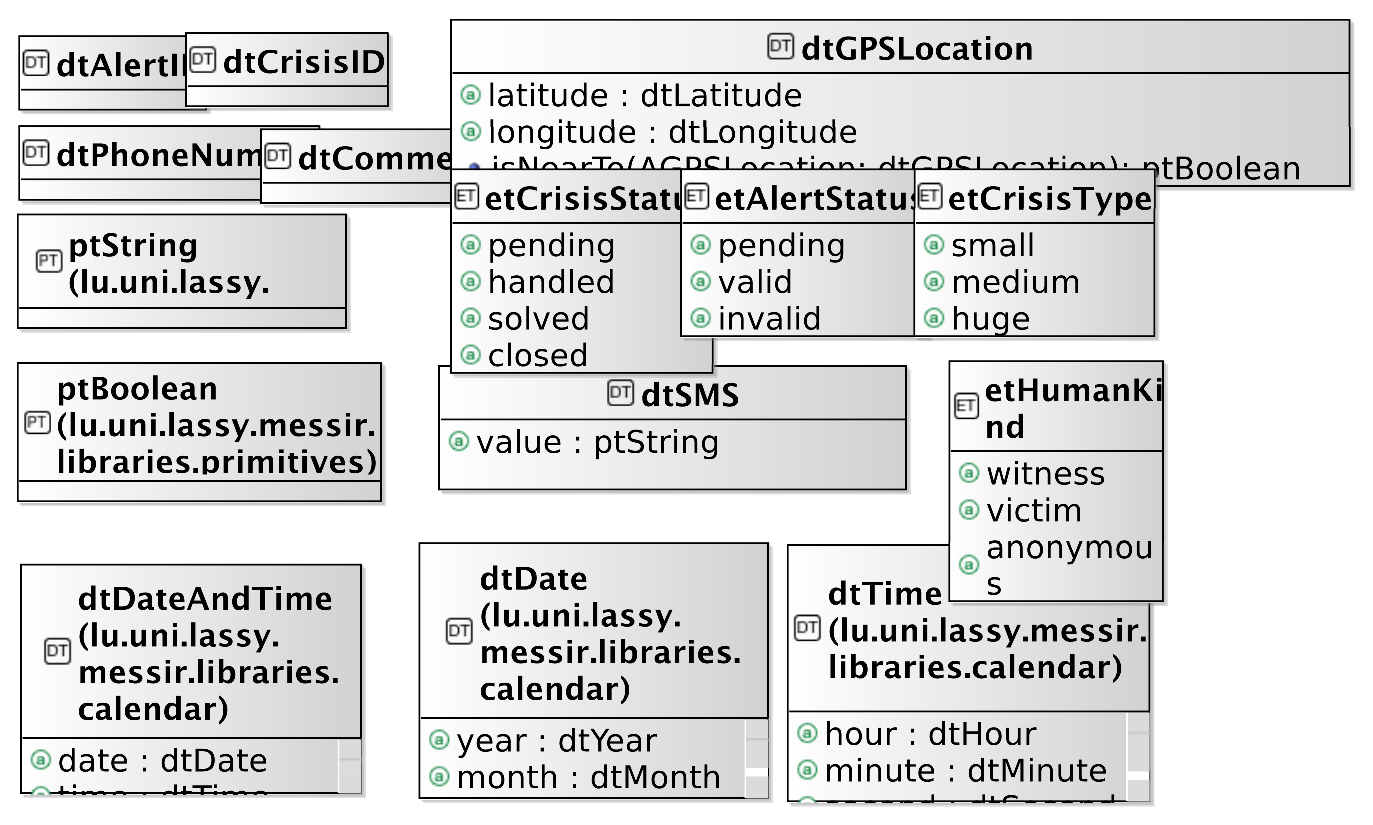
\includegraphics[
angle=0
,width=1.0\textwidth
]{./images-report-gen/operation-model/operation-scope-outactComCompany-oeAlertv2.eps}
\end{center}
\caption[lu.uni.lassy.excalibur.examples.icrash Operation Scope: operation-scope-outactComCompany-oeAlertv2]{oeAlert operation scope
}
\label{fig:lu.uni.lassy.excalibur.examples.icrash-OM-scopeView-operation-scope-outactComCompany-oeAlertv2}
\end{figure}
\vspace{0.5cm}

Figure \ref{fig:lu.uni.lassy.excalibur.examples.icrash-OM-scopeView-operation-scope-outactComCompany-oeAlertv3}
shows concept model elements in the scope of the oeAlert operation

\begin{figure}[htbp]
\begin{center}

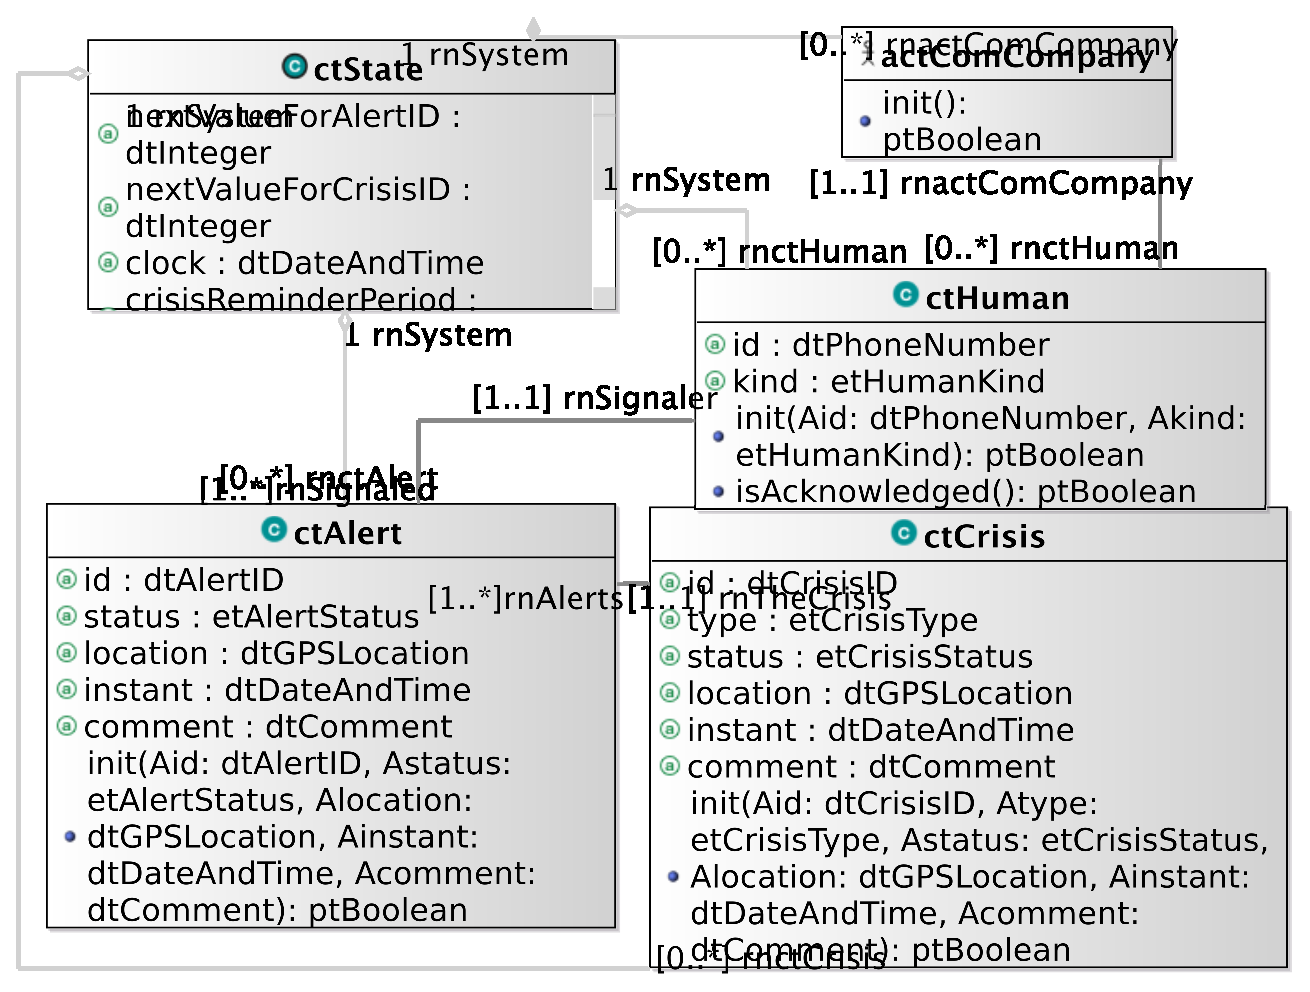
\includegraphics[
angle=0
,width=1.0\textwidth
]{./images-report-gen/operation-model/operation-scope-outactComCompany-oeAlertv3.eps}
\end{center}
\caption[lu.uni.lassy.excalibur.examples.icrash Operation Scope: operation-scope-outactComCompany-oeAlertv3]{oeAlert operation scope
}
\label{fig:lu.uni.lassy.excalibur.examples.icrash-OM-scopeView-operation-scope-outactComCompany-oeAlertv3}
\end{figure}
\vspace{0.5cm}

